\documentclass[11pt]{report}

\special{papersize=8.5in,11in}

\topmargin -0.5in \oddsidemargin 0.00in \evensidemargin 0.00in
\textwidth 6.75in \textheight 9.0in \headheight 0.25in \headsep
0.25in \footskip 0.5in \hoffset 0in \marginparpush 0.0in
\marginparwidth 0.0in \marginparsep 0.2in

\setcounter{page}{1}

\newcommand{\D}{\displaystyle}\newcommand{\T}{\textstyle}
\newcommand{\e}{{\mathrm{exp}}}
\newcommand{\dd}{{\mathrm d}}
\newcommand{\comment}[1]{}
\newcommand{\mb}{\mathbf}
\reversemarginpar

\usepackage[final]{graphicx}
\usepackage{fancyhdr}
%\graphicspath{{Papers/}}
\usepackage{amsthm,amssymb,amsmath}
\usepackage{cite}
\usepackage{geometry}
\usepackage{amsmath}
\usepackage{booktabs}
\usepackage{color}
\usepackage{setspace}
\usepackage{subfigure}
\usepackage{url}
%\usepackage[top=2.5cm, bottom=2.5cm, right=3.5cm, left=3.5cm]{geometry}
\geometry{a4paper,scale=0.8}
\setcounter{secnumdepth}{3}

\title{Research Progress Report}

\author{Botao Zhu}

\begin{document}
	
	\maketitle
	\lhead{\sf Research Progress Report - 2nd} \chead{} \rhead{\sf Botao Zhu}
	\lfoot{CTRG, University of Saskatchewan} \cfoot{} \rfoot{Page \thepage}
	\renewcommand{\footrulewidth}{1.0pt}
	\renewcommand{\headrulewidth}{2.0pt}
	\renewcommand{\arraystretch}{1.3}
	\pagestyle{fancy}
	
	\renewcommand{\thesection}{\arabic{section}}
	
	\section{Reading and Research Activities}
	

	\subsection{Reading Summary}
	\noindent\cite{Barbancho2007} introduces artificial intelligence algorithms into the wireless routing search by giving a Qos routing model based on neural networks to determine the quality of neighborhood. Compared with other routing protocols, like Directed diffusion and EAR, the proposed approach has a low level of delay with the increase of node numbers, because it can avoid to choose the failure intermediate nodes at the time of creating paths. And the average dissipated energy is also less than other methods.\\
	
	\noindent In order to deal with the increasing number of access terminals and exploding traffic, \cite{8254036} proposes a smart packet routing strategy with Tensor-based Deep Belief Architectures to predict the routing paths. It uses the tensor to model the input parameters, weights and biases. For input layer, it chooses the numbers of packets, corresponding time, source, destination and remaining buffer size to form a 5-dimensional array. And the output denotes the next node. The proposed deep learning model for routing search is shown in Algorithm 1.\\
	
	\begin{tabular}{lc}
		\toprule
		\textbf{Algorithm 1}
		\textbf{Input:} number of routers $N$, number of edge routers $E$, training data\\ (traffic pattern of edge routers, next router)\\
		\hline
		1: \textbf{for} each router $i\in N$ \textbf{to}\\
		2: \quad \textbf{for} each router $j\in E$ \textbf{do}\\
		3: \qquad Train the TDBA$\left[i\right]\left[j\right]$ with corresponding data\\
		4: \quad\textbf{end for}\\
		5: \quad Send the weight and bias values to the edge routers\\
		6: \textbf{end for}\\
		7: \textbf{for} each edge router $j\in E$ \textbf{do}\\
		8: \quad Record the traffic pattern $TP\left[j\right]$ and send it to other edge routers\\
		9: \quad Executive forward propagation process, output the next nodes\\
		10:\quad Use the next node information, construct the paths to destination routers\\
		11: \textbf{end for}\\
		12: \textbf{return} the paths to destination routers\\
		\hline
	\end{tabular}\\

	\noindent Compared with the OSPF, the proposed algorithm has a lower overhead and better performance in packet loss rate and average delay per hop.
	
	\subsection{A new Qos routing algorithm based on self-organizing maps for wireless sensor networks}
	\subsubsection{Designing the network topology}
	
	
	In order to cover a large area, communication strategy is needed. The authors consider a flat-based routing where all node have same roles. In general, the routes should be chosen so that nodes that are more critical for use as sensors are routed around as often as possible. The following sections will solve this problem.
	
	\subsubsection{Introducing neurons in sensor nodes}
	In WSNs, we usually use multi-hop schemes to transmit packets from source nodes to destination nodes and take some criteria to choose paths, such as minimum number of hops, minimum latency and minimum error rate, etc. In a special case, if all nodes want the paths to send packets to the base station, which can be solved by network backbone formation.\\
	
	\noindent The authors proposed a routing algorithm named Sensor Intelligence Routing (SIR) to form the network backbone. Assuming all the links in WSNs are symmetrical, the network can be modeled as an undirected graph $G:=\left(V,E\right)$. \\
	$w_{ij}$: the weight between the nodes $v_i$ and $v_j$.\\
	$d\left(v_i\right)$: the distance between the base station and a node.\\
	$\Gamma\left(v_i\right)=\left\{v_j\in V\mid\left(v_i,v_j\right)\in E\right\}$: the node $v_i$'s successor nodes.\\
	
	%To begin with, each node is initialized with a cost that should be updated by  the following steps. Considering the noisy environment, 
	\noindent How to evaluate the sensor network Qos? In this paper, each node is able to send a specific packet named ping to measure every neighbor link quality. So each node can obtain some parameters such as latency, error rate, duty cycle and throughput, which can from a four metrics to test the Qos levels. The link Qos parameters can be worked as the input of the neural network and the $qos$ values are the output, which can ensure to avoid the region with the worst quality and choose the dynamic paths for packets transmission. Equation $\left(1\right)$ is an example that the node $v_i$ calculates the distance to the root via the node $v_j$.\\ 
 	\begin{eqnarray}
 	d\left(v_i\right) = d\left(v_j\right)\times qos
 	\end{eqnarray}
	
	\noindent With regard to the neural network used in this paper, the authors choose the Self-Organizing Map (SOM) model\cite{58325}, which is an unsupervised neural network and has two layers architecture. The basic idea is that each neuron in the second layer of the network competes for an opportunity to respond to input parameters in the first layer, and finally only one neuron becomes the winner. This winning neuron represents the classification of input values. Model is shown in Figure~\ref{1stfig}. when inputting a vector, only the one whose vector most closely resembles the input vector can respond. After that, the winning neuron and  its neighboring neurons will update the weight. 
	\begin{figure}[h!]
		\centering
		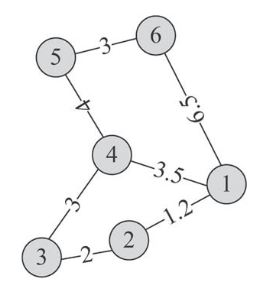
\includegraphics[width=0.5\linewidth]{figure1.jpg}
		\caption{SOM Architecture}
		\label{1stfig}
	\end{figure}
	
    \subsubsection{Training phase}
	The authors create several WSNs over OLIMPO \cite{1462037} with 250 nodes and different levels of data traffic. The node $v_i$ sends a ping packet to the node $v_j$ periodically and receives the acknowledgment, which can express the Qos environment by four metrics:latency, throughput, error rate and duty cycle. During this process, the noise power density $N_0$ and the distance $d$ should be considered. In order to obtain enough samples, this process is repeated 100 times with different $N_0$ and $d$. And then, these samples work as the input vectors of SOM and the output is several clusters. Each cluster, mapped to a neuron of the output layer, has similar characteristics and means a kind of Qos levels. For mathematizing the Qos, the authors define an output function $\Theta \left(i,j\right)$ with the values from 0 and 10 to represent the Qos levels. ({\color{red}Remark: this step should be supervised by an engineer according to the authors' description}). And also:\\
	\begin{eqnarray}
	qos = \Theta\left(i,j\right)
	\end{eqnarray}
	$\left(i,j\right)$ means the position of a neuron in the output layer. After the training phase finishes, the SOM is formed. 
	
	\subsubsection{Evaluating phase}
	To simulate one kind of scenarios without failure nodes, the authors create a wireless network with 250 nodes by OLIMPO. The node 0 is denoted as a sink and the node 22 is declared as a source. How to find the optimal routing from the node 22 to the node 0 is the most important problem. They choose two metrics, average dissipated energy and average delay, to evaluate the performance of SIR.
	\begin{itemize}
		\item Average dissipated energy means the energy consumption that a node deliver message to the sink. 
	\end{itemize}
	\begin{itemize}
		\item Average delay means the average one-way latency between transmitting an event and receiving it at each sink.
	\end{itemize}
 	\begin{figure}[h]
		\centering
		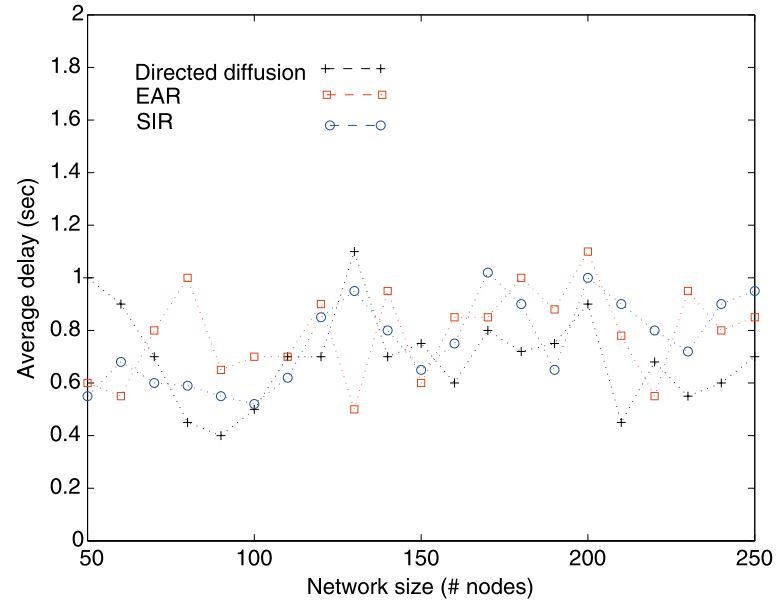
\includegraphics[width=0.5\linewidth]{figure2.jpg}
		\caption{Average latency}
		\label{1stfig}
	\end{figure}

	\begin{figure}[h]
		\centering
		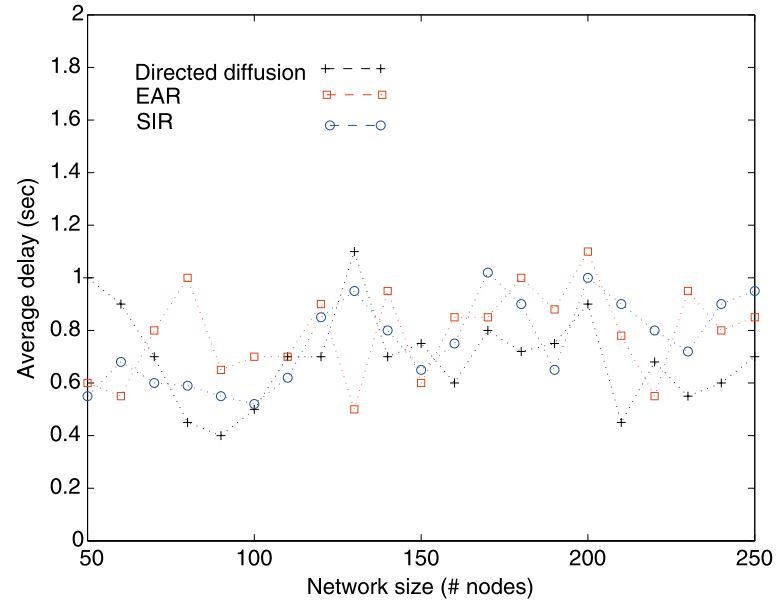
\includegraphics[width=0.5\linewidth]{figure2.jpg}
		\caption{Average dissipated energy}
		\label{1stfig}
	\end{figure}
   	\noindent The simulation is event-driven and assumes that the radio channel is symmetric. In order to compare the results, directed diffusion and EAR are used.
    
	\subsection{Code Summary}
	The basic idea of Low-energy Adaptive Clustering Hierarchy (LEACH) \cite{926982} is to select cluster head nodes randomly and distribute the load energy of the whole network to each node equally, so as to reduce the energy consumption of the network and improve the overall lifetime of the networks.\\
	
	\noindent LEACH performs clusters reconstruction circularly. Each round can be divided into two stages: the establishment of clusters and the stable stage. For the first stage, it includes four steps: the selection of cluster head node, the broadcasting of cluster head, the establishment of cluster head nodes and the generation of scheduling mechanism. The selection of cluster head nodes depends on the total number of cluster head nodes needed in the network and the number of times that each node has become a cluster head node so far. Each node randomly select a value between 0 and 1. If the value is less than a certain threshold, the node will become the head node of the cluster. And then, the head nodes will broadcast in the whole network. Other nodes will decide to join a specific cluster according to the signal strength of the received information and they will notify the corresponding head node to complete the establishment of the cluster. I use Matlab to simulate this protocol. In the region of $50m\times50m$, 100 points are distributed randomly. Figure~\ref{2ndfig} shows the number of dead nodes. Please see \textbf{leach1.m}.\\
	
	\begin{figure}[h!]
		\centering
		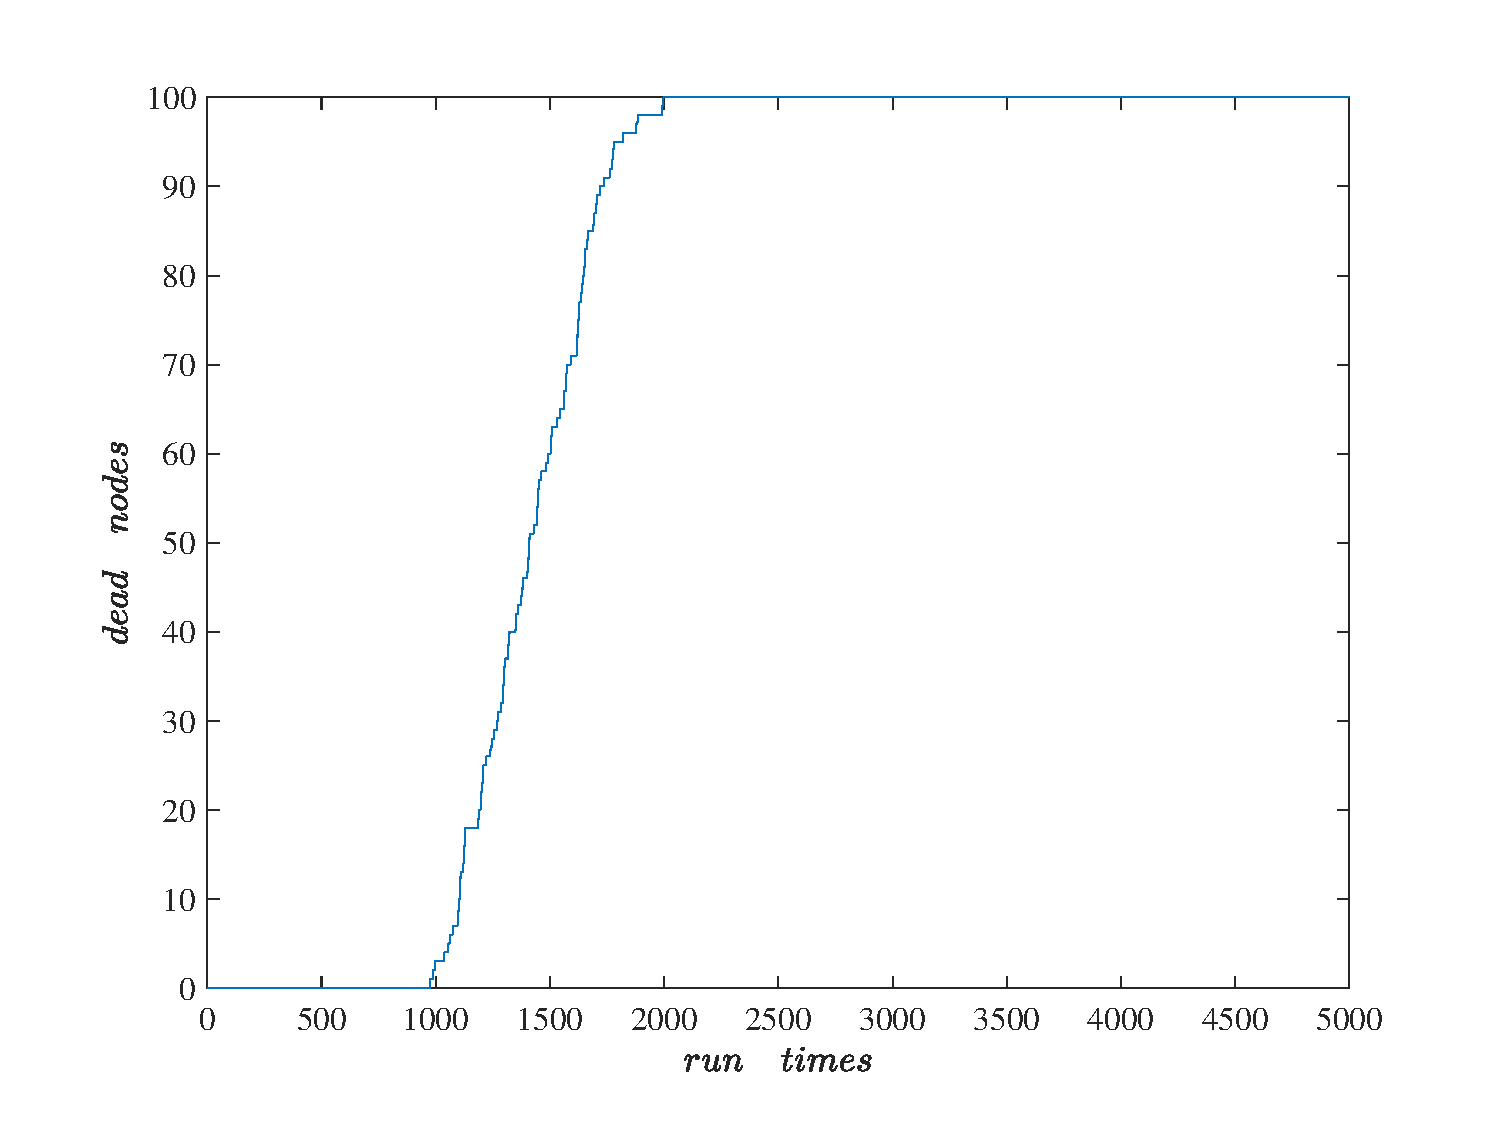
\includegraphics[width=0.4\linewidth]{leach.eps}
		\caption{The number of dead nodes}
		\label{2ndfig}
	\end{figure}
	\subsection{Course Summary}
	Studied chapter 1, chapter 2 and chapter 3 of Neural Network and Deep Learning.

	\section{Objectives for the Next 2 Weeks}
	\subsection{Reading} 
	Read papers foused on ML-based or DL-based routing. Draw the basic process of using machine learning to solve routing problems and investigate some simulation platforms in this field.
	\subsection{Course} 
	Study chapter 4 of Neural Networks and Deep Learning and chapter 1 of Improving Deep Neural Networks, \textbf{Coursera}, \url{https://www.deeplearning.ai/deep-learning-specialization/}
	
	\section{Advisor's Comments}
	
	\bibliographystyle{IEEEtran}
	\bibliography{janbib}
	
\end{document}